\section{Active Armrest}
\begin{figure}[h]
\centering
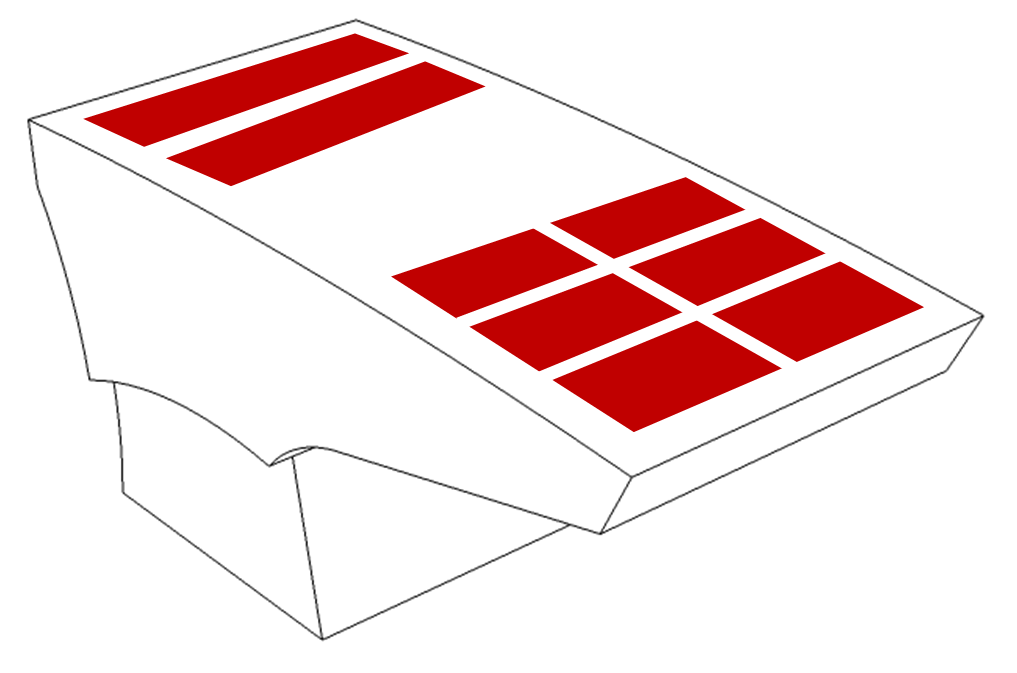
\includegraphics[width=0.4\textwidth]{images/active_armrest}
\caption{Active armrest sketch - six electrodes for finger gesture detection in front, two for arm detection in back}
\label{fig:armrest_sketch}
\end{figure}
The Active Armrest is a prototype to demonstrate unobtrusive gestural interaction in the domain of automotive applications [74]. The interior of modern cars can be considered a smart environment as it includes an ensemble of sensors and actors that adapt the system behavior according to user preference.
 
%Figure 24 Active armrest sketch - six electrodes for finger gesture detection in front, two for arm detection in back
Many cars use touch screens or jog dials to control primary and secondary car functions \cite{schmidt2010automotive}. Capacitive proximity sensors allow integrating interactive areas into different existing surfaces of a car, e.g. an armrest. The Active Armrest is using a set of eight sensors that are separated into two different groups. There are two larger electrodes in the back of the armrest that are dedicated to recognizing the presence of an arm. In the front of the armrest there is an array of six small electrode sensors, in order to register finger gestures, as shown in Figure \ref{fig:armrest_sketch}. The basic idea is to disallow interaction when the arm is resting and enable it once it's lifted. The Active Armrest supports swiping gestures of a single finger and static holding gestures of two fingers. This allows controlling various typical automotive applications, e.g. a navigation application, whereas holding is zooming in and out and swipe pan through the maps. Similar applications, such as multimedia features and comfort settings can be controlled in a similar fashion.
\subsection{Data processing}
\begin{figure}[h]
\centering
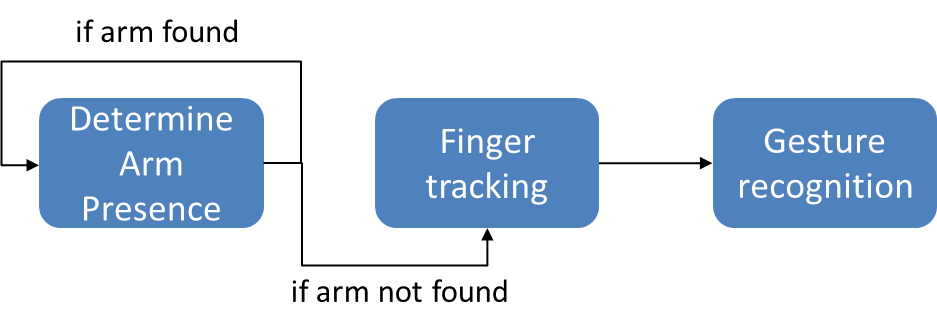
\includegraphics[width=0.4\textwidth]{images/armrest_dataproc}
\caption{Data processing pipeline of Active Armrest}
\label{fig:armrest_dataproc}
\end{figure}
%Figure 25 Data processing pipeline of Active Armrest
As we already mentioned, the Active Armrest electrodes are put into two groups. The data processing for both groups is distinctly different. In order to detect the presence of the arm using the two-electrode group a simple threshold on the accumulated values is used. The six sensor array in the front (touch area) is using the presented weighted average method to calculate finger positions. Additionally a threshold is used to distinguish one and two fingers. Overall there is a data processing pipeline as shown in Figure \ref{fig:armrest_dataproc}. The finger tracking and gesture recognition will be inactive until it is ensured that no arm is present. 
\subsection{Evaluation}
\begin{figure}[h]
\centering
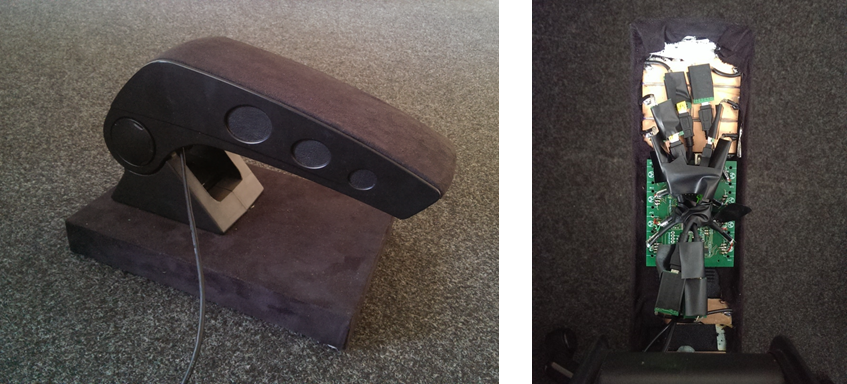
\includegraphics[width=0.8\textwidth]{images/armrest_proto}
\caption{Active Armrest prototype, left - outside view, right - detail view of electronics}
\label{fig:armrest_dataproc}
\end{figure}
%Figure 26 Active Armrest prototype, left - outside view, right - detail view of electronics
In order to evaluate the Active Armrest we have built the prototype shown in Figure \ref{fig:armrest_dataproc}. An aftermarket armrest was equipped with an OpenCapSense toolkit. The demonstration application is based on the SenseKit debug software supplied with the toolkit. As of now there is a simple USB connection to a nearby PC.
\begin{figure}[h]
\centering
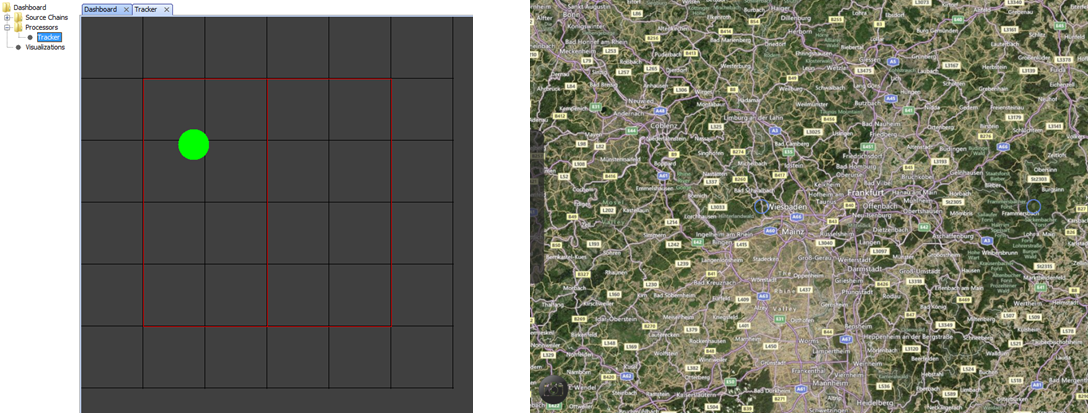
\includegraphics[width=0.6\textwidth]{images/armrest_eval}
\caption{Active Armrest demo software, left - finger tracker, right - OSM based navigation application}
\label{fig:armrest_eval}
\end{figure}
%Figure 27 Active Armrest demo software, left - finger tracker, right - OSM based navigation application
Figure \ref{fig:armrest_eval} shows a screenshot of the finger tracking application on the left, with a two-finger touch registered on the upper left part of the touch area. It is interfaced with a TUIO \cite{kaltenbrunner2005tuio} based maps application using OpenStreetMap \cite{haklay2008openstreetmap} data. The map is moved around using simple swipe movements of the finger that are directly associated to pan-features of the demonstration application. Zooming is activated by two-finger hold gestures on the upper or lower part of the touch area. We have used public displays of this prototype to get an idea of how easily unaffiliated persons learn to use the system. While the majority agreed on the potential of the application, there have been some reservations regarding the current gesture set, particularly that a closer relationship to smartphone touch screen gestures would be welcome.
